\clearpage\begingroup\SourceLeaf{31b}\HistoricalHead{26}{L}{PHYSIK. BRIEFWECHSEL.}
\begin{center}
[4.]\\[.7em]
\textsc{Gauss} an \textsc{Schumacher}. Göttingen, 14. Mai 1836.
\par\medskip\rule{.78\textwidth}{.35pt}\par
{\small [Briefwechsel zwischen \textsc{Gauss} und \textsc{Schumacher} III, Altona 1860, S. 57, 58.]}\par
\rule{.78\textwidth}{.35pt}
\end{center}
\noindent .\ .\ .\ .\ .\ .\ .\ .\ .\ .\ .\ .\ .\ .\ .\ .\ .\ .\ .\ .\ .
\par\noindent\hspace*{\parindent}Kann ich es demnächst möglich machen, so würde es mir sehr erwünscht
sein, wenn die Waage ganz hier bleiben könnte, obwohl ich in diesem Augenblick
hierüber noch nichts bestimmt sagen kann. Sehr lieb würde es mir
aber in diesem Fall sein, wenn die Waagebalken eine Eintheilung, wenn auch
nicht in einzelne Millimeter, doch etwa von 5 zu 5, oder von 10 zu 10 Millimeter
hätten. Würden solche durch die Art der Striche kenntlich gemacht,
z. B. dass etwa von 50 zu 50 Millimeter in die Augen fallende Unterschiede
das Zählen erleichtern, so könnten gravirte Zahlen wegbleiben, die ohnehin
sich wohl nicht mehr gut anbringen lassen. Der Vortheil, eine Eintheilung
zu besitzen, ist besonders, dass man von dem Besitz sehr scharfer ganz kleiner
Gewichtssätze unabhängig wird. Herr Prof. \textsc{Weber} hat in diesen Tagen
einen nur sehr rohen Versuch an einem hölzernen Waagbalken gemacht, den
er auf einer Theilmaschine getheilt, an die Theilungsstellen Nadeln eingefügt
hat, worüber mit Coconfäden ein etwa \(\frac{1}{3}\) Gramm schweres Laufgewicht gehängt,
und die Ausschläge wurden nach dem Reflexionsprincip (wie bei meinen
Magnetometern) mit einem Fernrohr an dem Spiegelbilde einer verticalen Scale
\clearpage\SourceLeaf{32}\HistoricalHead{27}{R}{GAUSS AN SCHUMACHER.}
\noindent aus einem Spiegel, der am Waagbalken befestigt war, beobachtet. Hier zeigte
sich die Wirkung des veränderten Moments, je nachdem das Laufgewicht von
einer oder von einer andern Nadel hing etc., mit äusserster Regelmässigkeit
fortschreitend, so dass Veränderungen, die (bei Belastung von \(\frac{1}{2}\) Kilogramm
in jeder Schale) nur dem Auflegen eines kleinen Bruchs eines Milligramms
in der Schale äquivalirten, mit Sicherheit zu erkennen waren, obgleich das
Ganze noch gar nicht einmal gegen Luftzug durch einen Kasten geschützt
war, sondern frei hing.

Ohne Herrn \textsc{Repsolds} Waage gesehen zu haben, kann ich freilich nicht
beurtheilen, welche Schwierigkeiten der Anbringung einer Eintheilung etwa
im Wege stehen können. Schwerlich wird der Waagebalken Metall für Eine
einzige gerade Linie darbieten, dann würde man freilich zufrieden sein müssen
\begin{center}
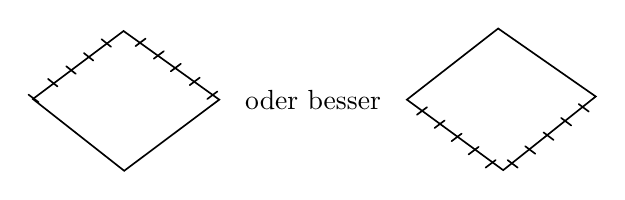
\begin{tikzpicture}[x=.008cm,y=-.008cm,line width=.6pt,line cap=round]
\draw (195,712)--(339,604)--(491,713)--(340,826)--cycle;
\draw (188,705)--(204,717) (219,680)--(234,692) (248,660)--(263,672) (276,639)--(291,651) (304,617)--(319,629);
\draw (358,628)--(374,616) (387,648)--(403,636) (414,668)--(430,656) (444,690)--(460,678) (472,712)--(488,700);
\node at (640,713) {oder besser};
\draw (789,713)--(934,600)--(1089,708)--(942,825)--cycle;
\draw (805,737)--(821,725) (833,758)--(849,746) (860,779)--(876,767) (887,800)--(903,788) (914,821)--(930,809);
\draw (949,809)--(965,821) (977,787)--(993,799) (1006,765)--(1022,777) (1034,742)--(1050,754) (1062,720)--(1078,732);
\end{tikzpicture}
\end{center}
\noindent zwei gebrochene gerade Linien zu haben, wo man dann suchen muss den
stumpfen Winkel zwischen beiden Linien anderweitig auszumitteln. Ist aber
Anbringung einer brauchbaren Theilung nicht praktikabel, so muss ich freilich
darauf (i. e. auf die Theilung) renonciren, und sehen, wie ich mir auf andere
Weise helfe, etwa durch Anbringung einer Scale auf einem polirten Glasstreifen
hinter der Waage.\quad .\ .\ .\ .
\clearpage\endgroup
